% 116-85(116쪽) — 좌표평면 위의 두 직선 $y=x$·$y=-x$ 와 점 $\pt{P_1}$ 에서 차례로 내린 수선의 발
% $\pt{P_2}$~$\pt{P_6}$(원문 「오른쪽 그림」). 스캔 화질이 낮아 TikZ 로 다시 그림.
% 라벨은 원문 것만: $x$, $y$, $\pt{O}$, 두 직선 이름, $\pt{P_1}$~$\pt{P_6}$. 수선의 발마다 직각 표시를 둔다.
% 선분의 길이는 적지 않는다 — 어느 선분이 길이 $\left(\frac{1}{2}\right)^8$ 인지(답)가 그림에서 읽히지 않게.
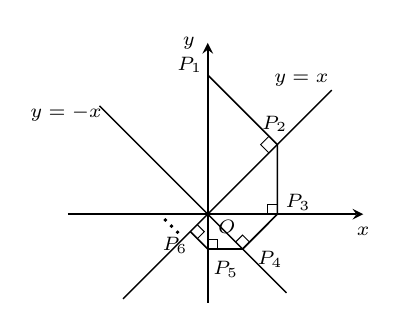
\begin{tikzpicture}[x=1.25cm, y=1.25cm, line width=0.6pt, >=stealth]
  \draw[->, line width=0.7pt] (-1.42,0) -- (1.58,0) node[below=1pt, font=\scriptsize] {$x$};
  \draw[->, line width=0.7pt] (0,-0.90) -- (0,1.74) node[left=1pt, font=\scriptsize] {$y$};
  \draw[line width=0.5pt] (-0.86,-0.86) -- (1.26,1.26) node[anchor=south east, inner sep=1pt, font=\scriptsize] {$y=x$};
  \draw[line width=0.5pt] (-1.10,1.10) -- (0.80,-0.80);
  \node[anchor=east, inner sep=1pt, font=\scriptsize] at (-1.04,1.02) {$y=-x$};
  % 수선의 발을 차례로 이은 선
  \draw (0,1.414) -- (0.707,0.707) -- (0.707,0) -- (0.354,-0.354) -- (0,-0.354) -- (-0.177,-0.177);
  % 직각 표시
  \draw[line width=0.35pt] (0.622,0.792) -- (0.537,0.707) -- (0.622,0.622);
  \draw[line width=0.35pt] (0.707,0.100) -- (0.607,0.100) -- (0.607,0);
  \draw[line width=0.35pt] (0.425,-0.283) -- (0.354,-0.212) -- (0.283,-0.283);
  \draw[line width=0.35pt] (0.100,-0.354) -- (0.100,-0.254) -- (0,-0.254);
  \draw[line width=0.35pt] (-0.106,-0.248) -- (-0.035,-0.177) -- (-0.106,-0.106);
  % 계속됨을 나타내는 원문의 점 세 개
  \foreach \t in {1,2,3}{\fill (-0.245-0.062*\t,-0.245+0.062*\t) circle (0.020);}
  \node[anchor=south east, inner sep=1pt, font=\scriptsize] at (-0.02,1.40) {$\pt{P_1}$};
  \node[anchor=south, inner sep=1pt, font=\scriptsize] at (0.68,0.80) {$\pt{P_2}$};
  \node[anchor=west, inner sep=1.5pt, font=\scriptsize] at (0.74,0.12) {$\pt{P_3}$};
  \node[anchor=west, inner sep=1pt, font=\scriptsize] at (0.47,-0.46) {$\pt{P_4}$};
  \node[anchor=north west, inner sep=1pt, font=\scriptsize] at (0.02,-0.44) {$\pt{P_5}$};
  \node[anchor=north east, inner sep=1pt, font=\scriptsize] at (-0.17,-0.20) {$\pt{P_6}$};
  \node[anchor=north west, inner sep=1pt, font=\scriptsize] at (0.07,-0.02) {$\pt{O}$};
\end{tikzpicture}
